\subsection{High Frequency Simulation Software}

The simulations software used is Ansys HFSS (High Frequency Simulation Software). HFSS uses a numerical technique, namely the Finite Element Method (FEM). FEM divides the problem space into small elements, each of which have an assigned function. Those so-called basis functions are weighted, and together they represent the real field solution. 


It solves for \autoref{eqn:full_wave_equation}, where $\epsilon_r$ is the relative permeability and $\mu_r$ is the relative permeability of the material. The variable $k_0$ is the wave number of free space and equals $k_0=\omega\sqrt{\epsilon_0\mu_0}$. \cite{Cendes_Lee_1988,Lee_Sun_Cendes_1991,Cendes_1991}.

\begin{equation}
    \nabla\times\left(\frac{1}{\mu_r}\nabla\times\mathbf{E}\right)-k_0^2\epsilon_r\mathbf{E}=0 \quad\text{in $\Omega$}
    \label{eqn:full_wave_equation}
\end{equation}

This equation is solved in a computational domain $\Omega$. This computational domain is divided into finite elements, called a mesh. Each mesh contains polynomial functions, which are weighted to approximate the real solution. It has been proven that tetrahedral finite elements are best suited for this task, as they are geometrically flexible and make the definition of complete polynomial approximation functions possible \cite{Shenton_Cendes_1985}. Ansys HFSS uses a adaptive finite element mesh generator, which automatically provides a mesh for a given 3-dimensional construction. \autoref{fig:tetrahedral_mesh} shows one of such tetrahedrons. At the edge points, the components of the field which are normal to the respective edge is stored. At the vertex points, the component of a field which are tangential to the edges are stored. The value of the field at any midpoint is derived through interpolation from the node values.

\begin{figure}[h]
    \centering
    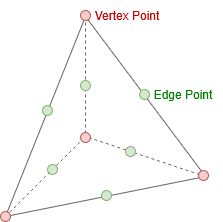
\includegraphics[width=0.25\linewidth]{Documentation/content/10_theory/img/tetrahedral_mesh.png}
    \caption{Tetrahedron with points on the edge and vertices.}
    \label{fig:tetrahedral_mesh}
\end{figure}

A testing function $W_n$ is defined, which is multiplied to \autoref{eqn:full_wave_equation}. Integrating over the whole test volume then leads to \autoref{eqn:test_funct}. This yields $N$ equations, with $n=1,2,...N$, for each finite element in the domain $\Omega$.

\begin{equation}
    \int_\Omega\left( W_n\cdot\nabla \times\left( \frac{1}{\mu_r}\nabla\times\mathbf{E} \right)-k_0^2\epsilon_rW_n\cdot\mathbf{E} \right)\mathrm{d}V=0
    \label{eqn:test_funct}
\end{equation}

Using the vector identy $\nabla\cdot\left(\mathbf{a}\times\mathbf{b}\right)=\left(\nabla\times\mathbf{a}\right)\cdot\mathbf{b}-\mathbf{a}\cdot\left(\nabla\times\mathbf{b}\right)$  on \autoref{eqn:test_funct} provides a weak form of the equation, meaning a form of the original partial differential equation, which does not contain all original derivatives \cite{Cendes_Lee_1988,Cendes_1991}. Additionally, boundary terms come into play, as seen in the right hand side of the resulting \autoref{eqn:greens_theorem_wave_eqn}. 

\begin{equation}
    \int_\Omega \left[ \left(\nabla \times W_n \right)\cdot \frac{1}{\mu_r}\nabla\times \mathbf{E}-k_0^2\epsilon_rW_n\cdot\mathbf{E}\right]\mathrm{d}V=\underbrace{\oint_{\partial\Omega}\left( W_n\times \frac{1}{\mu_r}\nabla\times\mathbf{E}\right)\cdot\mathrm{d}\mathbf{S}}_{\text{Boundary term}}
    \label{eqn:greens_theorem_wave_eqn}
\end{equation}

Next, the electric field $\mathbf{E}$ is represented by a superposition of basis functions. When applying Galerkin's method, the basis functions are equal to the test functions $W_n$. \autoref{eqn:representation_e_field_fem} demonstrates the sum of the basis functions, which are weighted with the variable $x_m$. These variables $x$ for all elements have to be solved, to find the electric field $\mathbf{E}$ over the whole domain. The FEM has therefore reduced the initial wave equation in \autoref{eqn:full_wave_equation} to a simple linear matrix equation $Ax=b$, where $A$ is a known $N\times N$ matrix, $b$ contains port excitations and $x$ is the unknown. The other electromagnetic quantities can be derived through the electric field.

\begin{equation}
    \mathbf{E}=\sum^N_mx_mW_n
    \label{eqn:representation_e_field_fem}
\end{equation}



Ansys HFSS (High Frequency Simulation Software) % Fehlende Ressourcen von Zoltan in Journal of Applied Physics. Schreibe über mathetmaische Grundlagen, Meshing, Dipole Excitation und Impedance Network Boundary Counditions (INBC)

% Additional missing ressource: Finite Elements, Electromagnetics, and Design


